\documentclass[11pt]{article}
\usepackage[utf8]{inputenc}
\usepackage[margin=0.8in]{geometry}
\geometry{a4paper}
\linespread{0.925} %全局行距

\usepackage{amsmath}
\usepackage{amssymb}
\usepackage{amsthm}
\usepackage{amsfonts}
\usepackage{comment}
\usepackage{booktabs}
\usepackage{array}
\usepackage{paralist}
\usepackage{verbatim}
\usepackage{fancyvrb}
\usepackage{multirow}
\usepackage{rotating}
\usepackage{fancyhdr}
\pagestyle{fancy} %全文使用的pagestyle
\renewcommand{\headrulewidth}{0pt}
\lhead{}\chead{}\rhead{}
\lfoot{}\cfoot{\thepage}\rfoot{}
\usepackage{sectsty}
\allsectionsfont{\sffamily\mdseries\upshape}
\usepackage{algorithm}
\usepackage{algpseudocode}
\usepackage[section]{placeins} %图片


\usepackage{natbib}
\bibliographystyle{abbrvnat}
\usepackage{filecontents} %允许把bib写在tex里

\usepackage{titlesec} %标题类型
\titleformat{\section}[display]
{\large\bfseries}{}{}{}[]

\usepackage{titlesec} %标题类型
\titleformat{\subsection}[display]
{\bfseries}{}{}{}[]


\usepackage{CJKutf8}
\usepackage{cprotect}
\usepackage{booktabs}
\usepackage[dvipsnames]{xcolor} %代码高亮+ref额外颜色
\usepackage[toc,title,titletoc]{appendix} %附录

\usepackage{graphicx}
\usepackage{float}%设置图片浮动位置
\usepackage[labelformat=simple]{subcaption} %更先进的子图包
\renewcommand\thesubfigure{(\alph{subfigure})}

\usepackage{hyperref}
\hypersetup{
	colorlinks=true,%会取消边框
	linkcolor=blue,
	filecolor=cyan,
	urlcolor=magenta,
	anchorcolor=red,
	citecolor= Green
}
%%% 比较丑的Python

\setlength{\parindent}{0em} %段首不缩进
\setlength{\parskip}{1ex} %段间空一行

\definecolor{codegrey}{HTML}{F8F8F8}
\usepackage{listings} %插入代码

\lstdefinestyle{lfonts}{
  basicstyle   = \footnotesize\ttfamily,
  stringstyle  = \color{purple},
  keywordstyle = \color{blue!60!black}\bfseries,
  commentstyle = \color{olive},
}
\lstdefinestyle{lnumbers}{
  numbers     = none,
  numberstyle = \tiny,
  numbersep   = 1em,
  firstnumber = 1,
  stepnumber  = 1,
}
\lstdefinestyle{llayout}{
  breaklines       = true,
  tabsize          = 2,
  columns          = fullflexible,
  backgroundcolor = \color{codegrey},
}
\lstdefinestyle{lgeometry}{
  xleftmargin      = 0pt,
  xrightmargin     = 0pt,
  frame            = tb,
  framesep         = \fboxsep,
  framexleftmargin = 0pt,
}
\lstdefinestyle{lgeneral}{
  style = lfonts,
  style = lnumbers,
  style = llayout,
  style = lgeometry,
}
\lstdefinestyle{python}{
    language = {Python},
    style    = lgeneral,
}


\title{Monthly Summary (January 2023)}
\author{CID: 02242799}
\date{}
\begin{document}
\begin{CJK}{UTF8}{gbsn}
\maketitle


\section*{Selection of $m_c$}

We use the Maximum Curvature (MaxC) method to select the value of $m_c$. The MaxC technique (\cite{wyss1999quantitative}; \cite{wiemer2000minimum}) is a fast and straightforward way to estimate $m_c$. It consists in defining the point of the maximum curvature by computing the maximum value of the first derivative of the frequency-magnitude curve and matching the magnitude bin with the highest frequency of events in the non-cumulative frequency-magnitude distribution.\citep{mignan2012estimating} Via this method, the $m_c$ value we obtained for this period is $m_c=0.3$ and the histogram of earthquake magnitude of the last 12 months is shown in Figure \ref{fig:s1} below.

\begin{figure}[h]
  \centering
  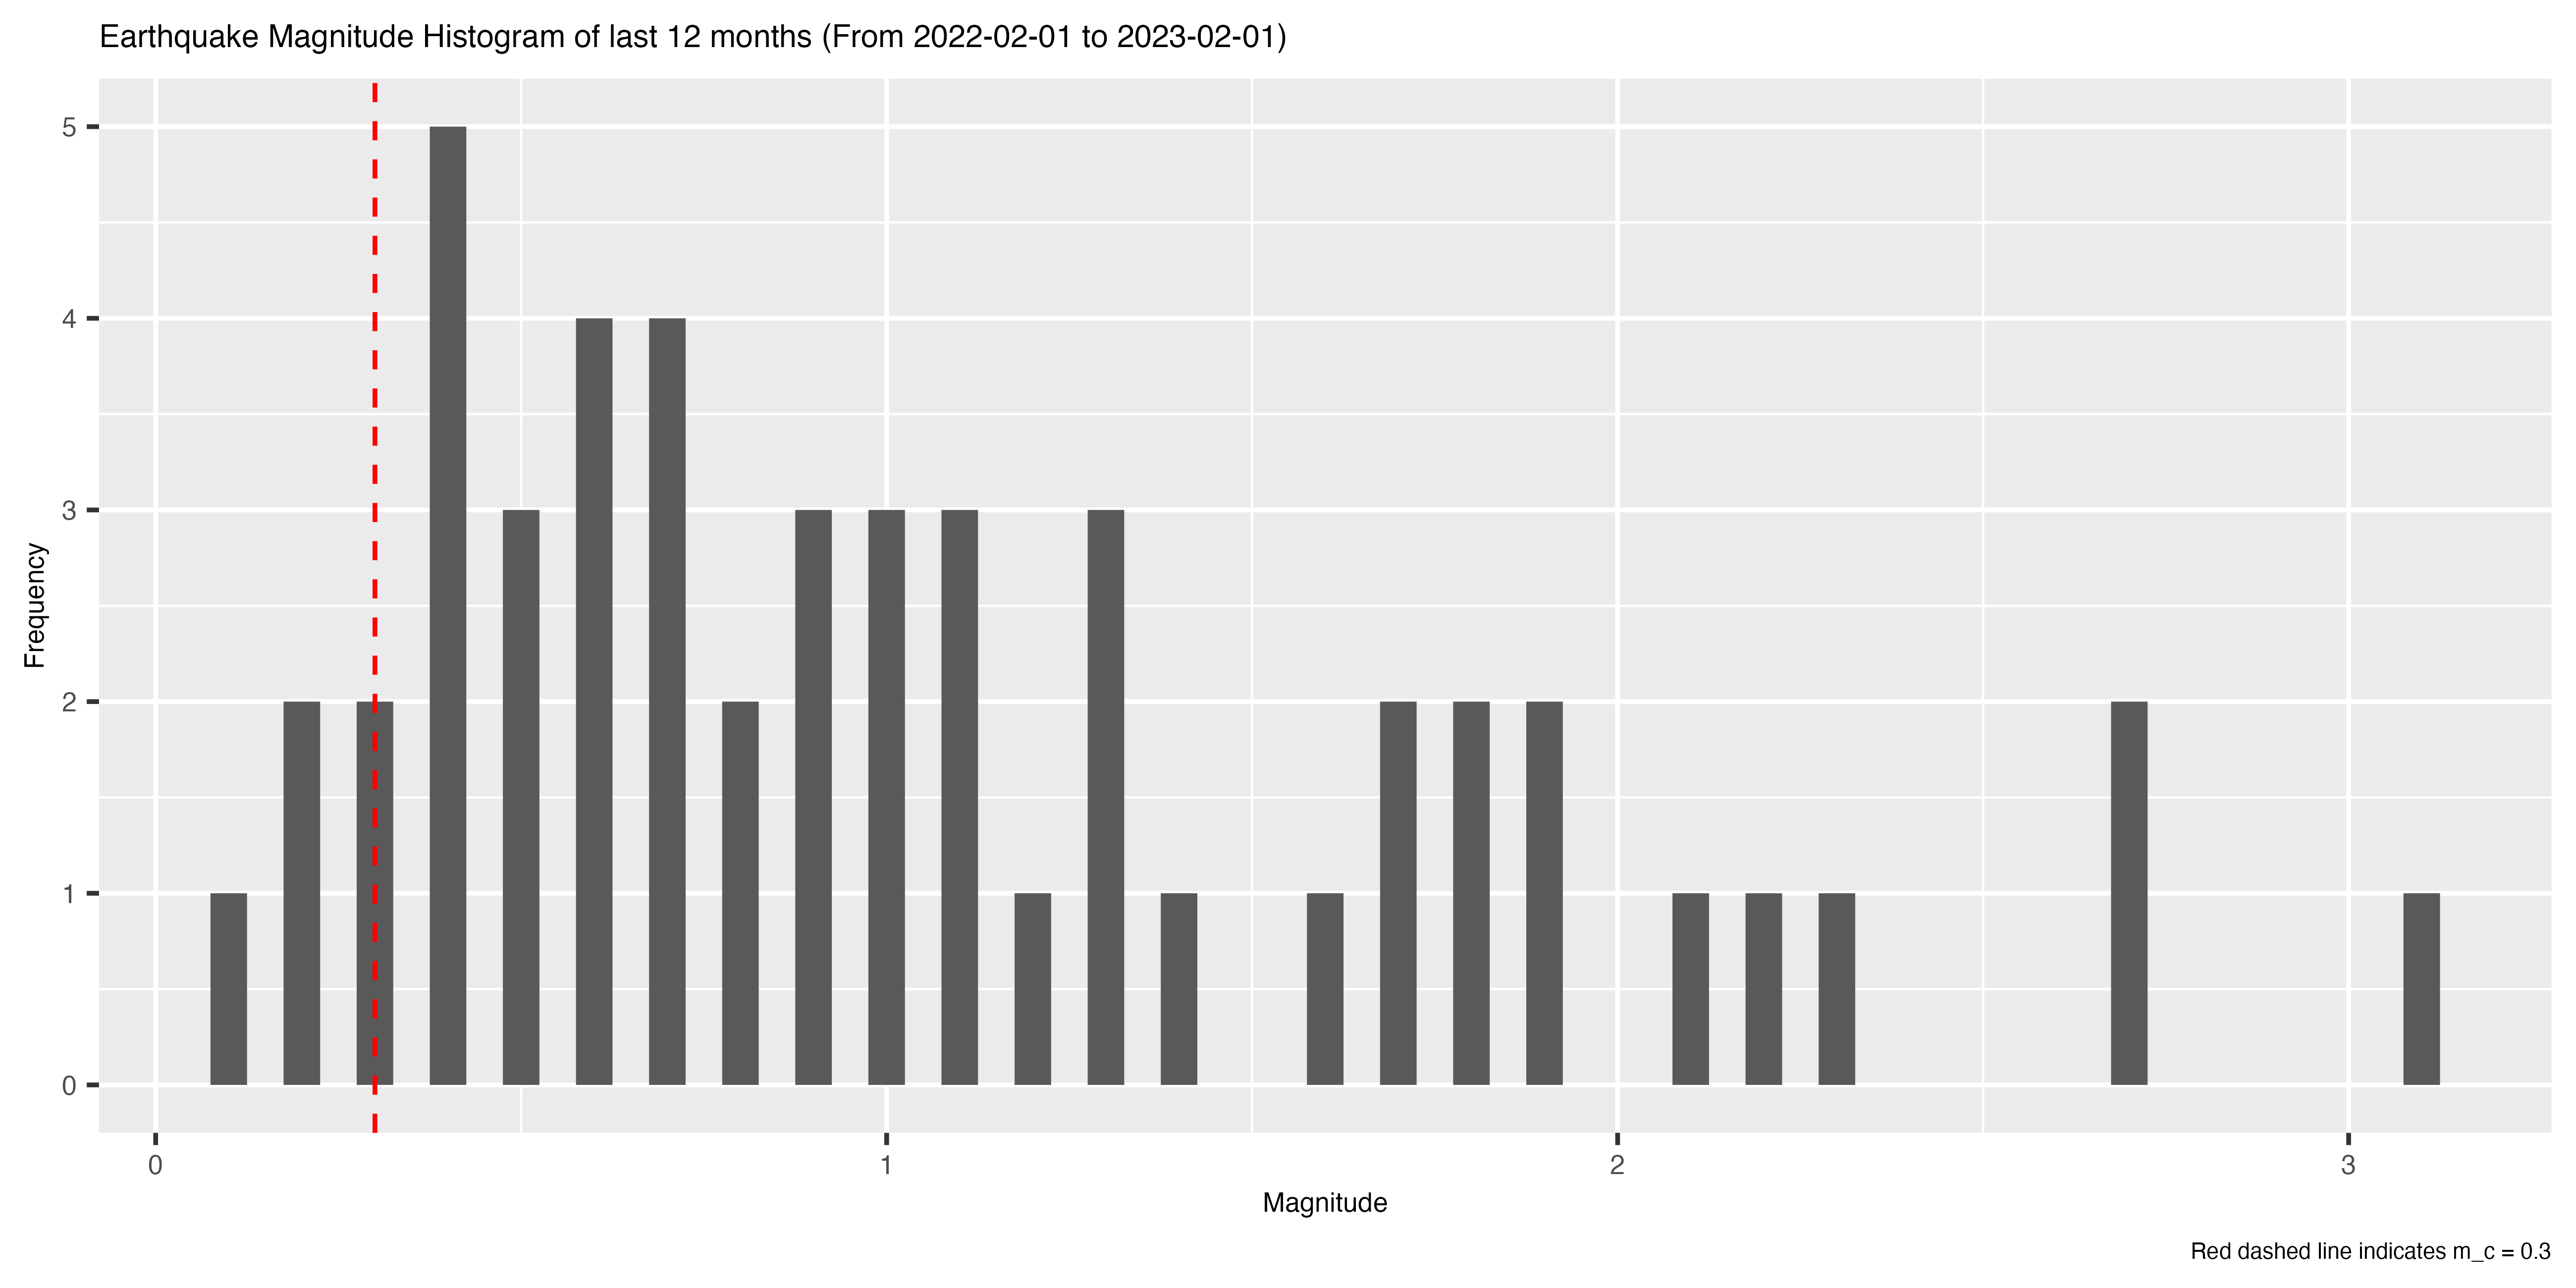
\includegraphics[height=6cm]{../../outputs/mag_hist.png}
  \caption{Earthquake Magnitude Histogram of last 12 months}
  \label{fig:s1}
\end{figure}

To validate our assumption of earthquake magnitude following an exponential distribution, we carry out a Kolmogorov-Smirnov test on the data values above $m_c$. The test yields a $p$-value of $0.6489$, which, being significantly higher than $0.05$, implies a strong similarity between the observed and expected data. Figure \ref{fig:s2} illustrates this comparison via the empirical cumulative distribution function (CDF) and the theoretical CDF for the exponential distribution. The close proximity between these two CDF curves further reaffirms the hypothesis that our data aligns well with the exponential distribution.

\begin{figure}[h]
  \centering
  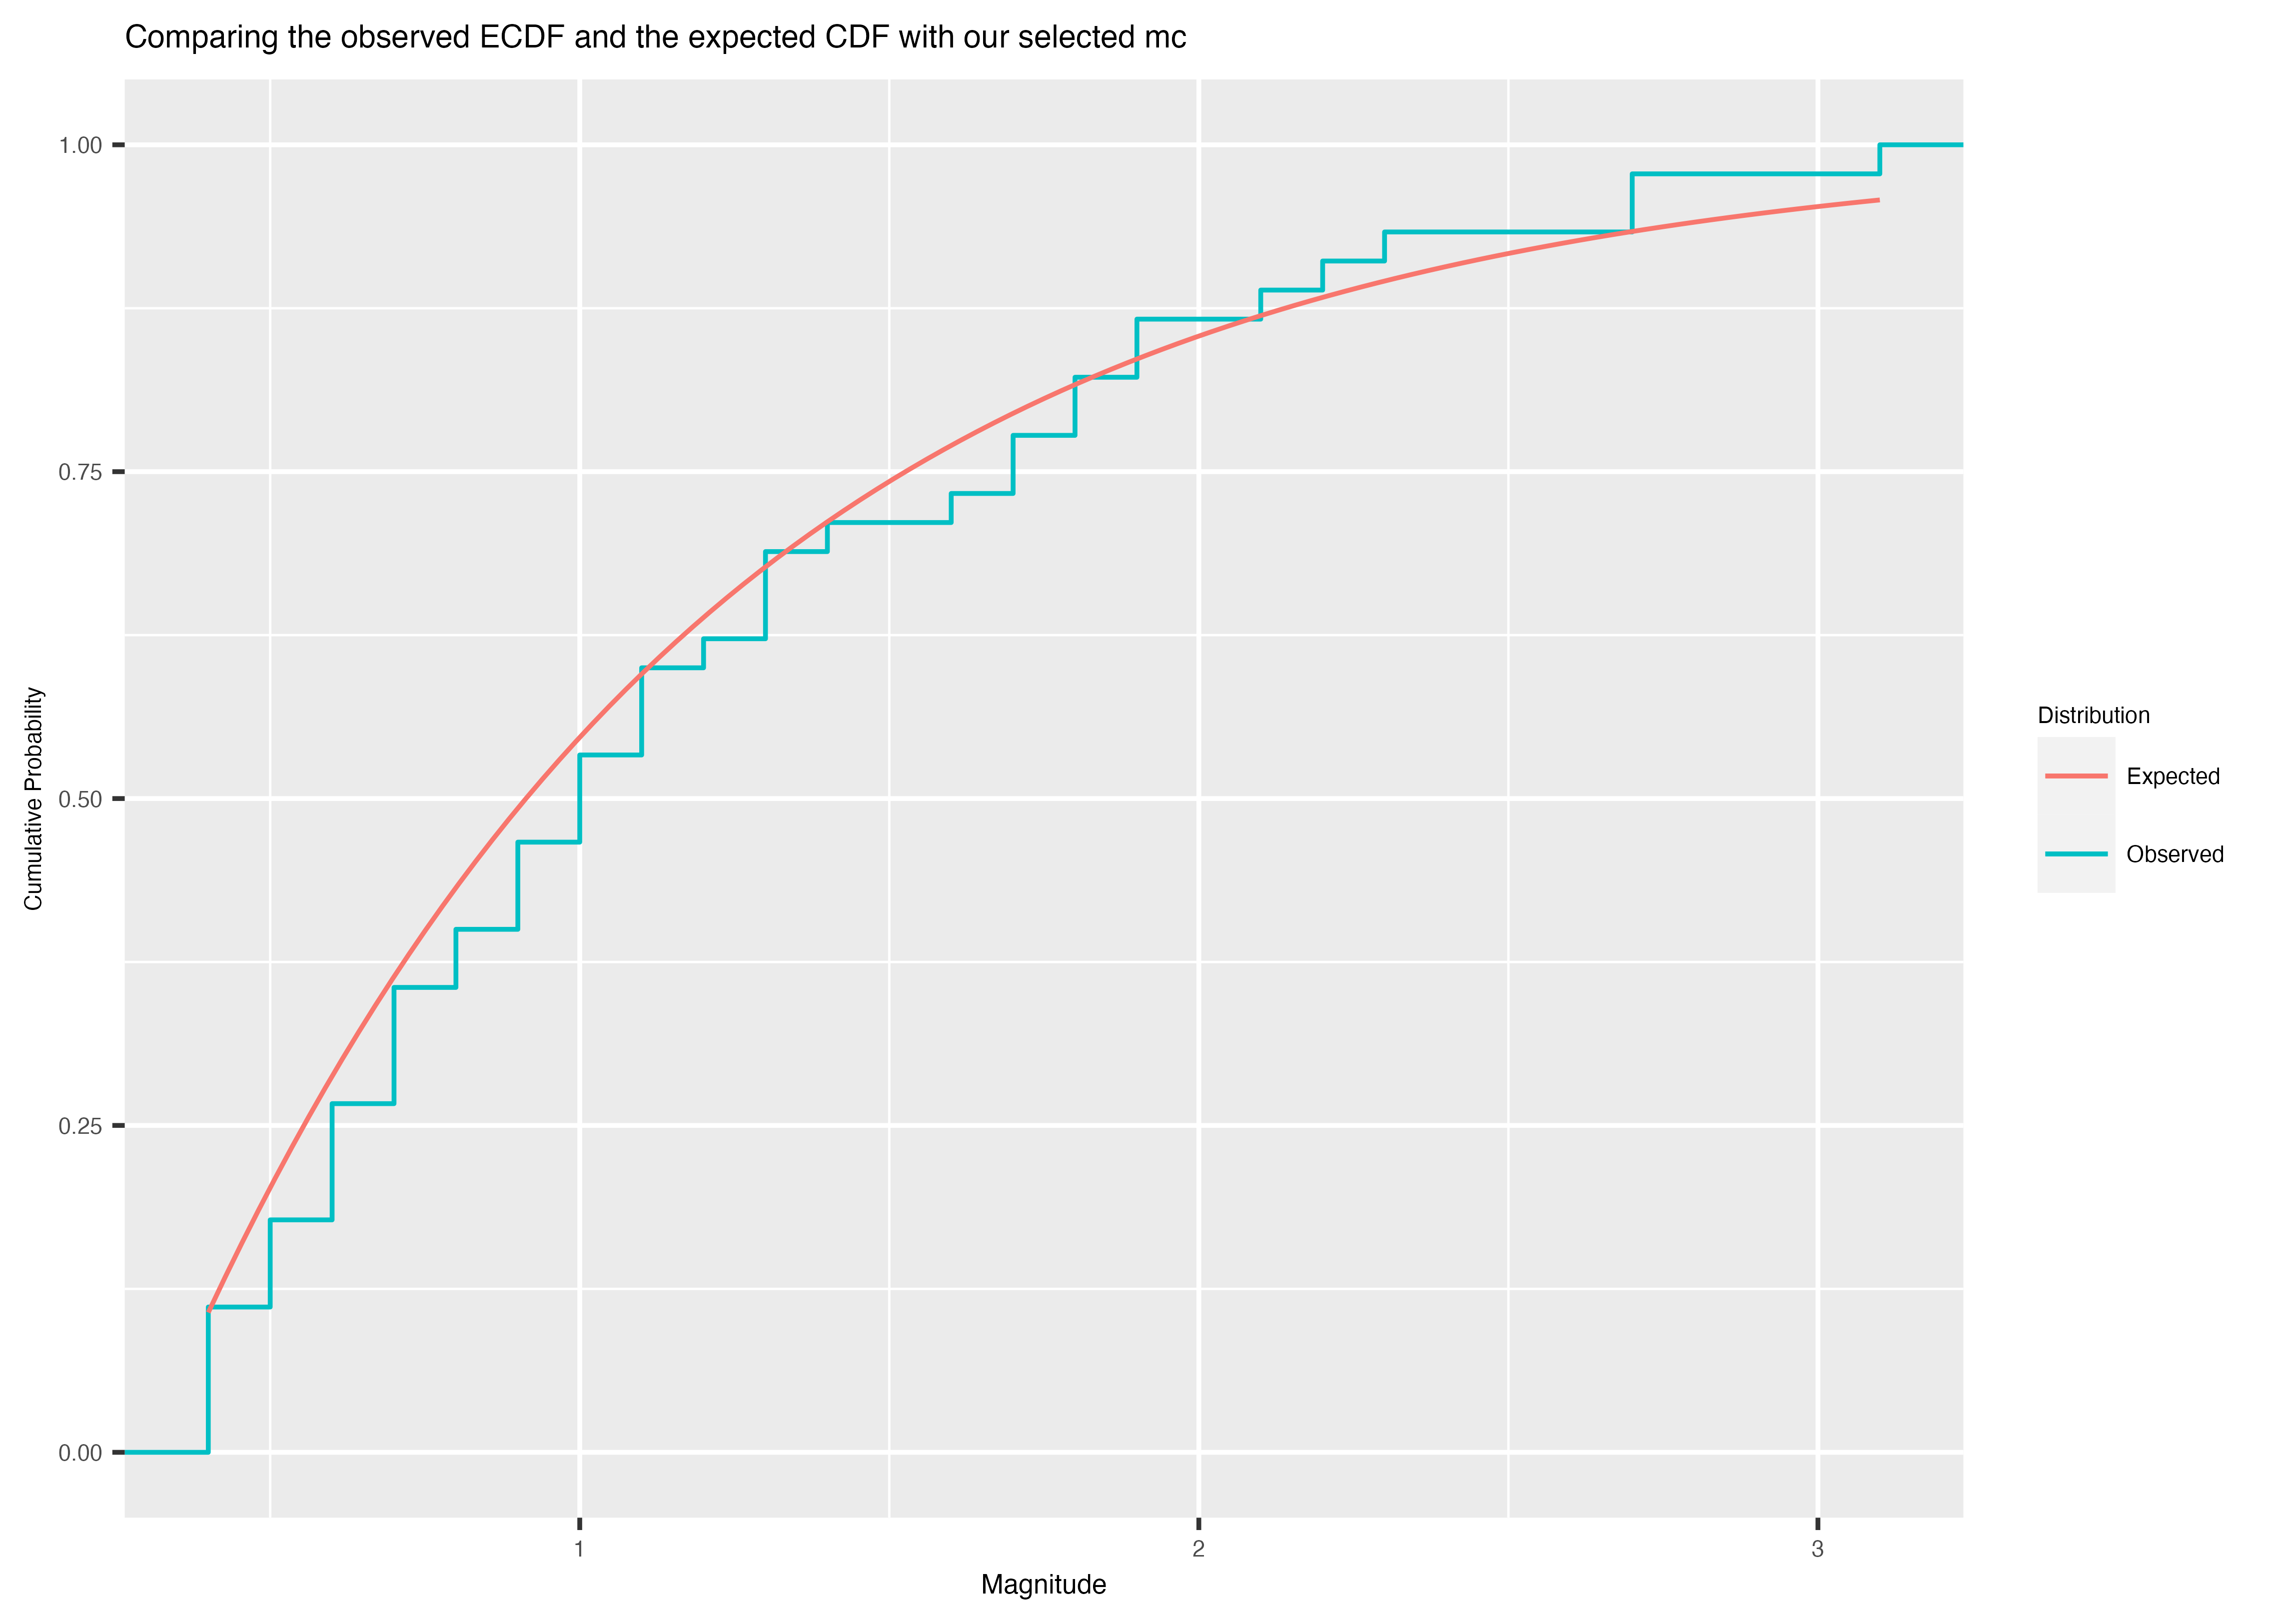
\includegraphics[height=5.4cm]{../../outputs/com_cdf_plot.png}
  \caption{Comparing the observed ECDF and expected CDF}
  \label{fig:s2}
\end{figure}



\section*{Compare the earthquake activity of last month and the previous 11 months}

There were 3 earthquake activities in the last month, while the average number of earthquake activities in the previous 11 months was 4.27. We plot a bor plot to visualise it as shown in Figure \ref{fig:2-1}. We also plot a box plot and a table to show the overall earthquake magnitude behaviour of the two periods as shown in Figure \ref{fig:2-2} and Table \ref{Tab:1}. We can observe that the mean magnitude is lower than average behaviour, but the median value is higher. The range of the magnitude seems similar to the previous.


\begin{figure}[h]
	\centering
    \begin{subfigure}{0.45\linewidth}
        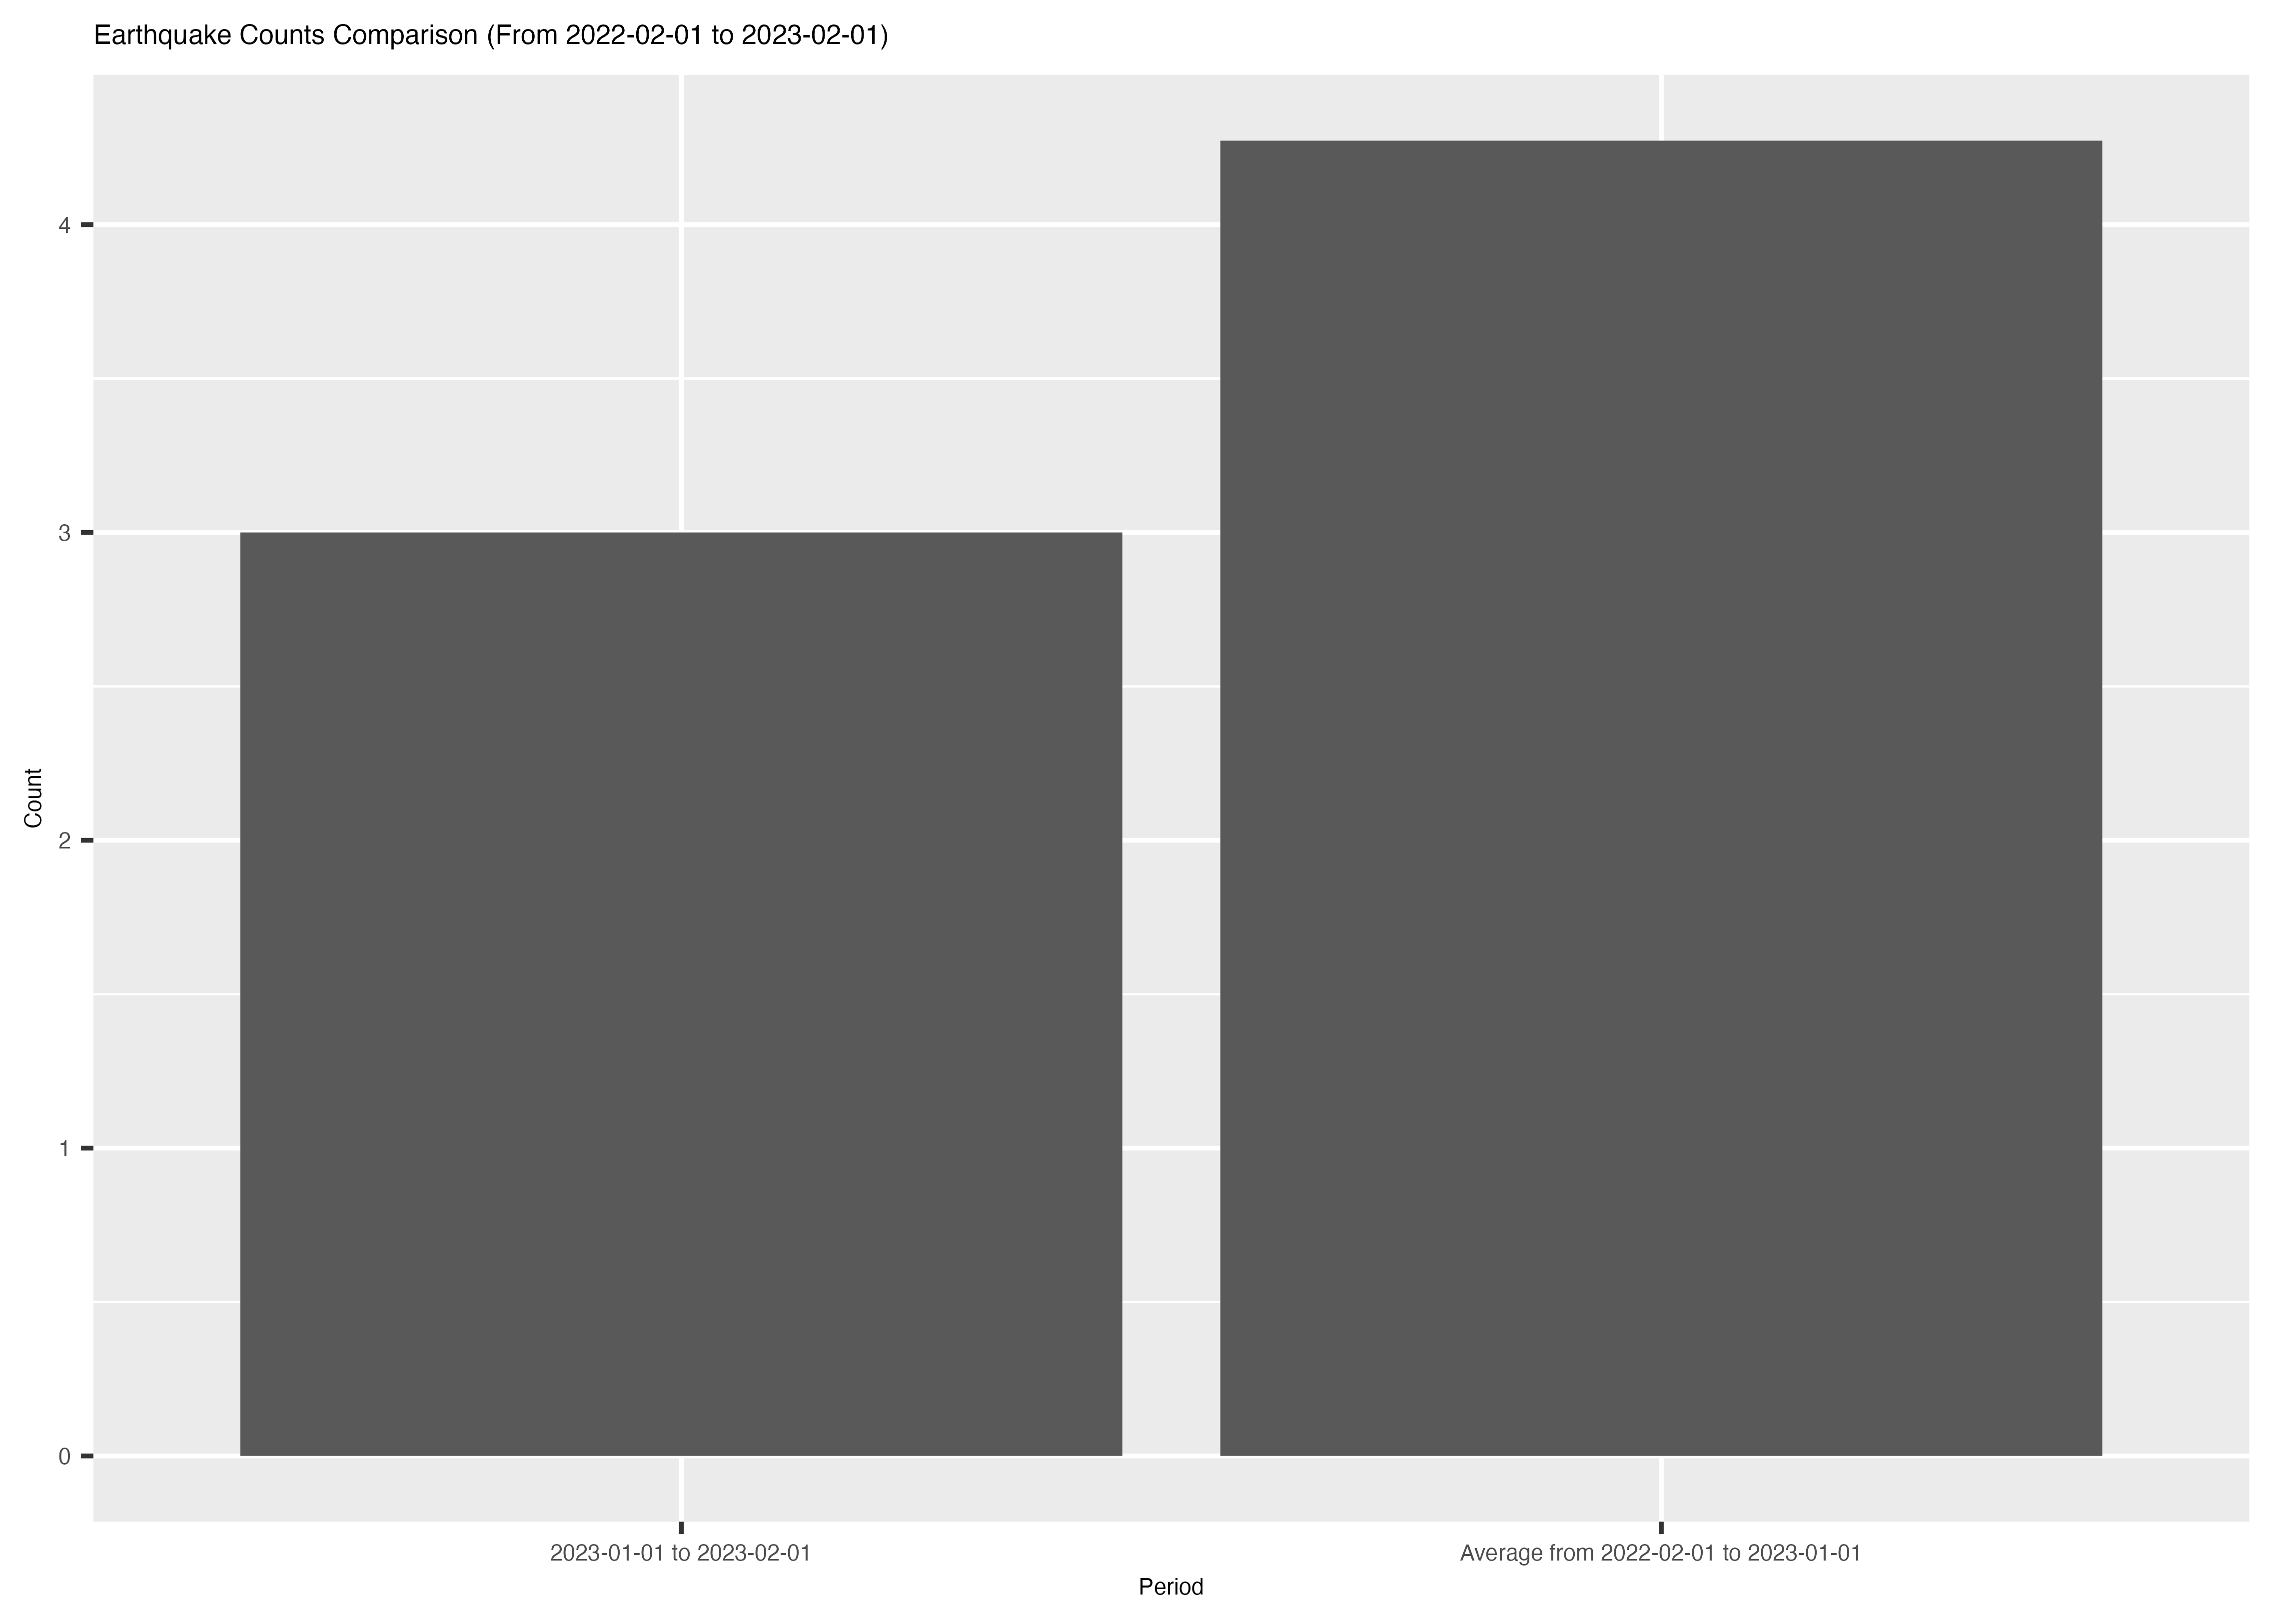
\includegraphics[width=8.75cm]{../../outputs/com_count_bar.png}
        \caption{Earthquake counts comparision}
        \label{fig:2-1}
    \end{subfigure}
    \hfill
    \begin{subfigure}{0.5\linewidth}
        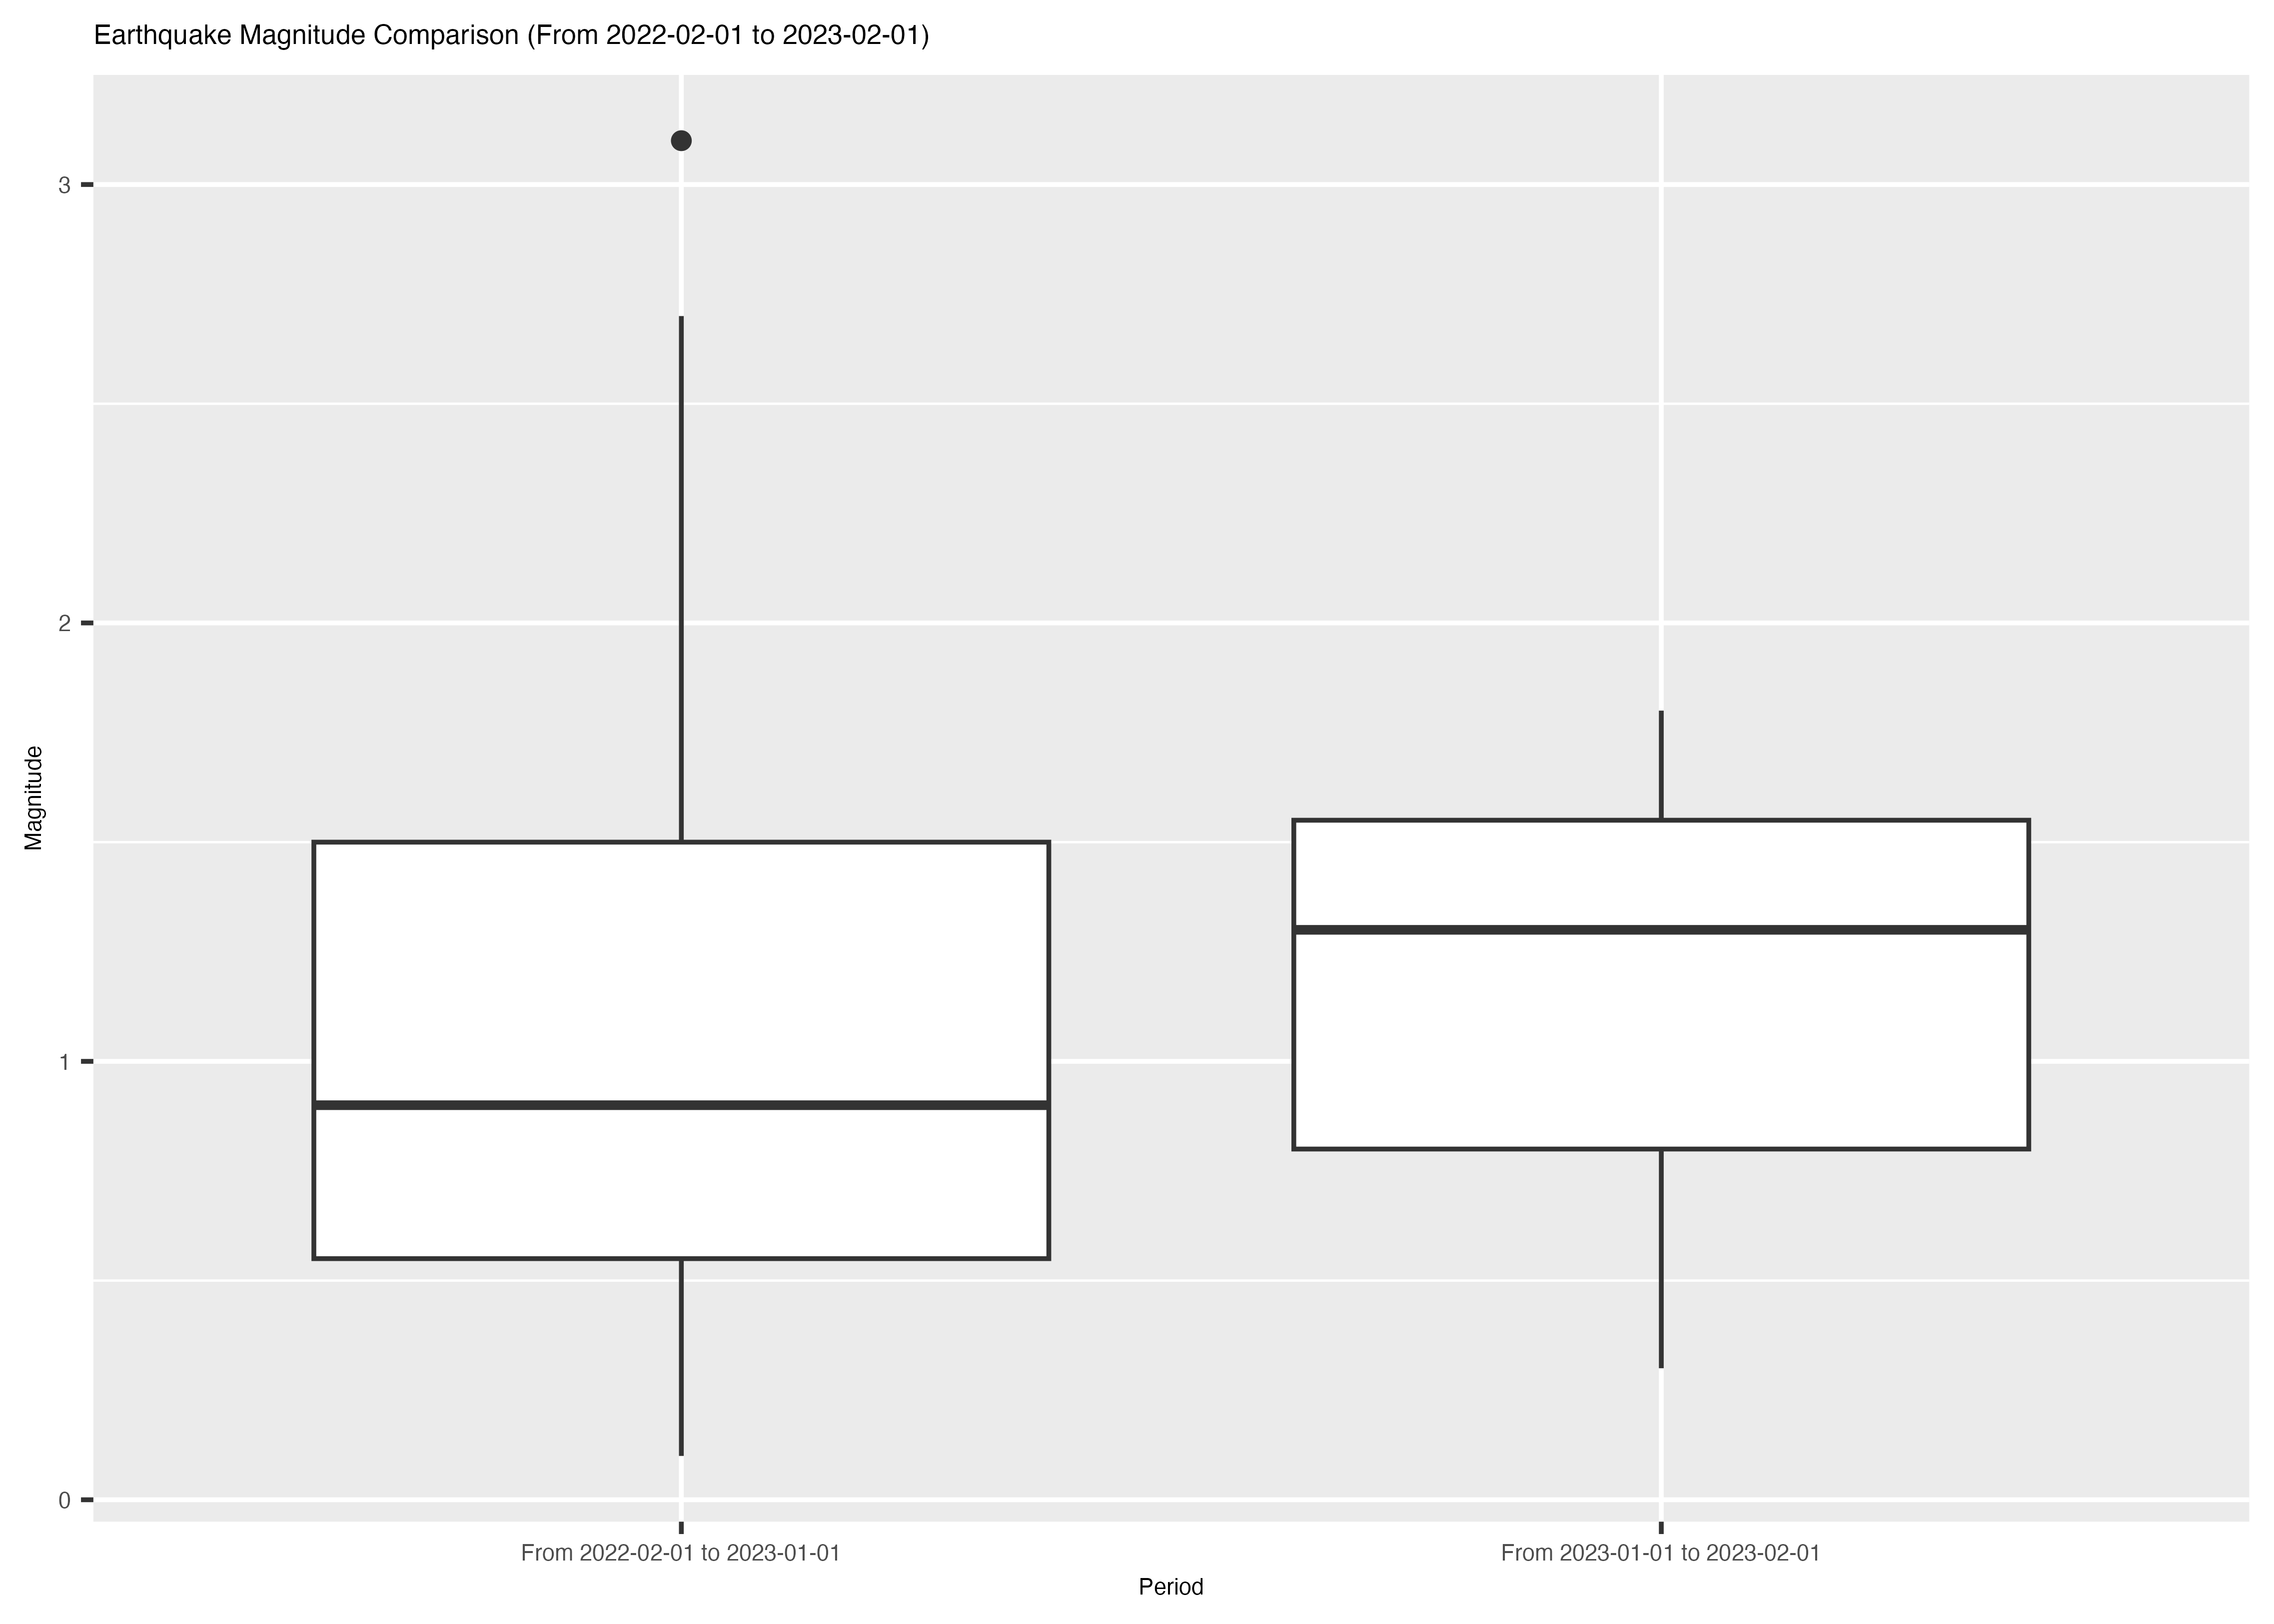
\includegraphics[width=8.75cm]{../../outputs/com_mag_box.png}
        \caption{Earthquake magnitude comparision}
        \label{fig:2-2}
    \end{subfigure}
    \caption{Comparision plots of counts and magnitude of the last month and previous 11 months }
    \label{fig:2}
\end{figure}

\begin{table}[h]
\begin{tabular}{c|cccccc}
                  & Min   & 1st Qu.        & Median & Mean  & 3rd Qu. & Max   \\ \hline
Last month        & 0.300 & 0.800          & 1.300  & 1.133 & 1.550   & 1.800 \\
Previous 11 months & 0.100 & 0.550 & 0.900  & 1.085 & 1.500   & 3.100
\end{tabular}
\centering
\caption{The summary statistics of the magnitude of last month and previous 11 months}
\label{Tab:1}
\end{table}

We also plot the location of the earthquake that happened last month with the location in the previous 11 months, as shown in Figure \ref{fig:c1}. There are two earthquakes that occurred in the same place, and they overlapped. Therefore there are only 2 points shown in the previous month. The earthquake location that happened last month is close to the place that happened in the previous 11 months.

\begin{figure}[h]
  \centering
  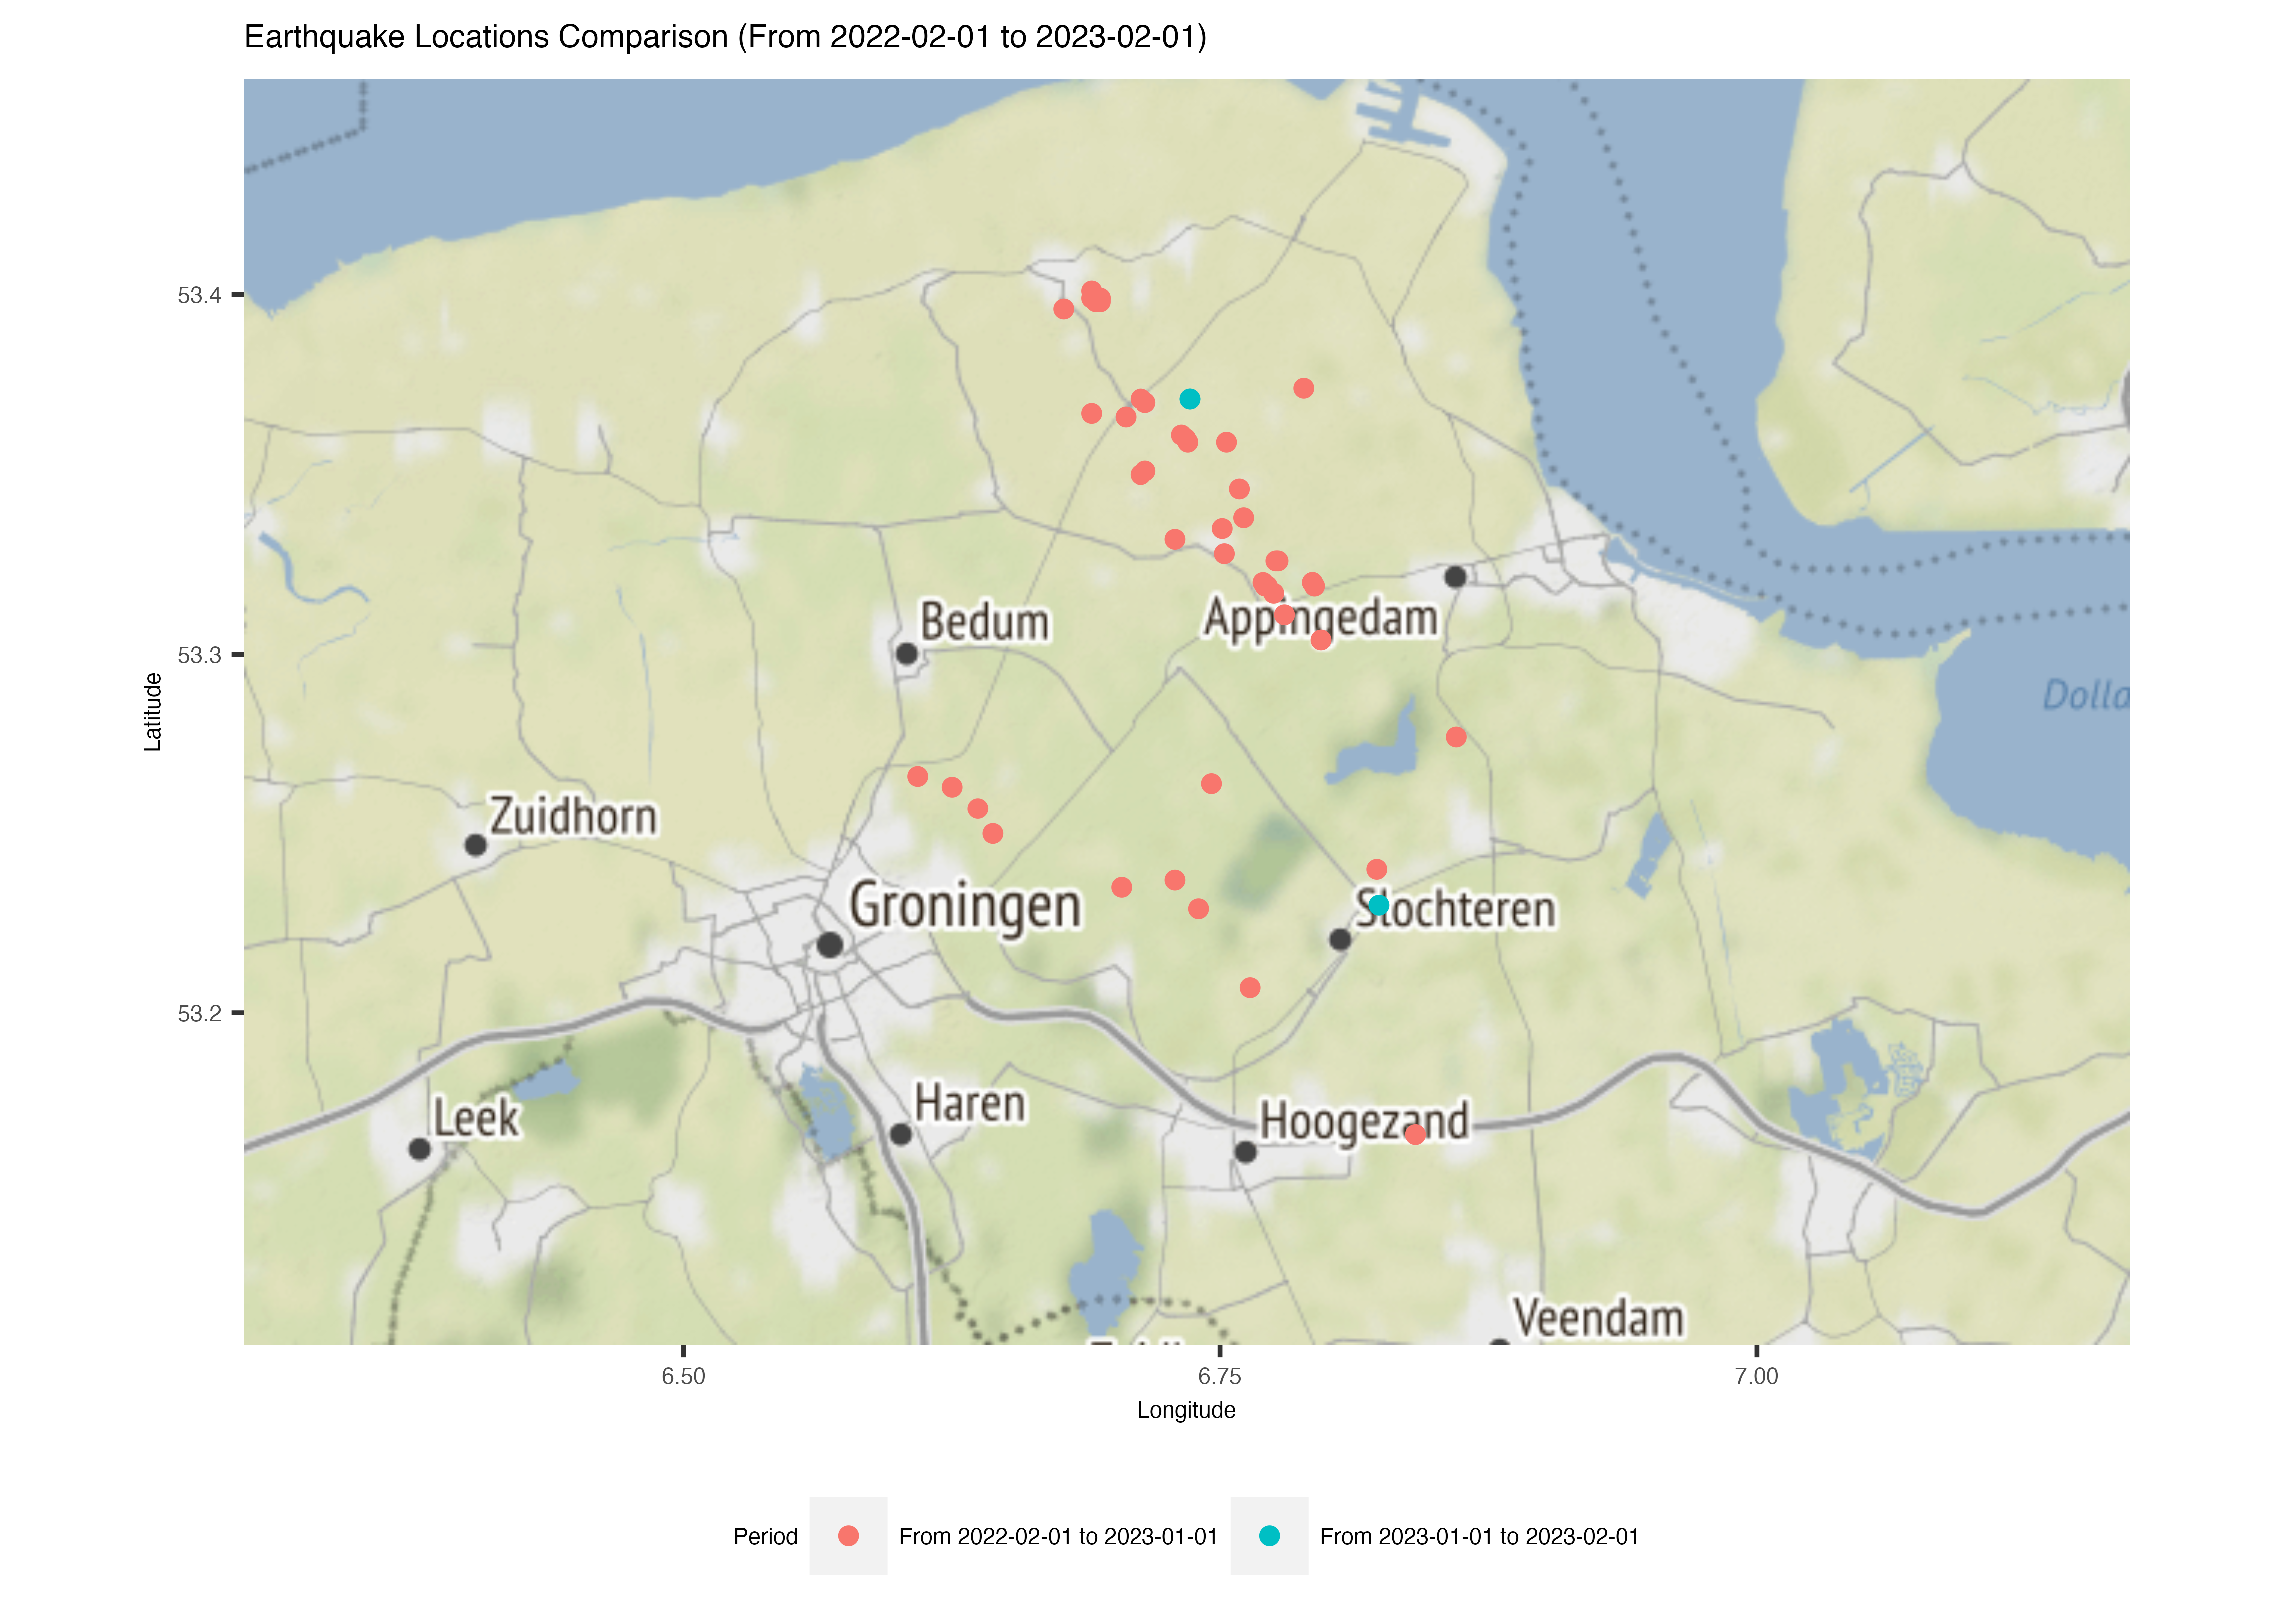
\includegraphics[height=7cm]{../../outputs/com_loc_plot.png}
  \caption{Comparing the earthquake location of last month and the previous 11 months}
  \label{fig:c1}
\end{figure}




\clearpage



\bibliography{\jobname} 


\begin{filecontents}{\jobname.bib}
@article{wyss1999quantitative,
  title={Quantitative mapping of precursory seismic quiescence before the 1989, M 7.1 off-Sanriku earthquake, Japan},
  author={Wyss, Max and Hasegawa, Akira and Wiemer, Stefan and Umino, Norihito and others},
  year={1999}
}

@article{wiemer2000minimum,
  title={Minimum magnitude of completeness in earthquake catalogs: Examples from Alaska, the western United States, and Japan},
  author={Wiemer, Stefan and Wyss, Max},
  journal={Bulletin of the Seismological Society of America},
  volume={90},
  number={4},
  pages={859--869},
  year={2000},
  publisher={Seismological Society of America}
}
@article{mignan2012estimating,
  title={Estimating the magnitude of completeness for earthquake catalogs},
  author={Mignan, Arnaud and Woessner, Jochen},
  journal={Community Online Resource for Statistical Seismicity Analysis},
  pages={1--45},
  year={2012},
  publisher={Community Online Resource for Statistical Seismicity Analysis}
}
\end{filecontents}

\end{CJK}
\end{document}




